\documentclass[dvipsnames]{article}
\usepackage{tikz,pgfplots}
\usepackage{tikz-qtree}
\usepackage{units}
\usepackage{braket}
\usepackage[]{xcolor}
\pgfplotsset{compat=1.14}
%\pgfplotsset{colormap={mix}{
%	color(0cm)=(blue);
%	color(1cm)=(green);
%	color(2cm)=(yellow)
%	color(3cm)=(red)}}

\usetikzlibrary{patterns,shadows,fadings,positioning,trees,calc}
\usepgfplotslibrary{external}
\tikzexternalize


\tikzfading[name=fade inside,
         inner color=transparent!80,
         outer color=transparent!30]
\tikzfading[name=fade out,
         inner color=transparent!0,
         outer color=transparent!90]


%\definecolor{diplom1}{rgb}{0.0 0.4 1.0}
%\definecolor{diplom2}{rgb}{0.0 0.0 0.6}
\definecolor{diplom1}{RGB}{101 156 239}
\definecolor{diplom2}{RGB}{000 000 128}
\definecolor{diplom3}{RGB}{153,0,0} %unirot
\definecolor{diplom4}{RGB}{232,215,23}
\definecolor{diplom5}{RGB}{51,37,60}

\definecolor{unirot}{RGB}{153,0,0}
\definecolor{unirot_hell}{RGB}{255,228,225}
\definecolor{lightblue}{RGB}{242.2,249.88,255}

\pgfplotsset{colormap={diplom1s}{
       color(0cm)=(white);
       color(1cm)=(diplom1);
       color(10cm)=(diplom1)}}
\pgfplotsset{colormap={diplom2s}{
       color(0cm)=(white);
       color(1cm)=(diplom1);
       color(2cm)=(diplom2)}}
\pgfplotsset{colormap={blues}{
       color(0cm)=(diplom2);
       color(1cm)=(diplom1);
       color(2cm)=(white);
       color(3cm)=(diplom1);
       color(4cm)=(diplom2)}}

\pgfplotsset{
   /pgfplots/bar cycle list/.style={/pgfplots/cycle list={%
        {diplom1,  fill=diplom1!30!white,  mark=none,very thick},%
        {diplom2,  fill=diplom2!30!white,  mark=none,very thick},%
        {diplom3,  fill=diplom3!30!white,  mark=none,very thick},%
        {orange,   fill=orange!30!white,   mark=none,very thick},%
        {LimeGreen,fill=LimeGreen!30!white,mark=none,very thick},%
        {Fuchsia,  fill=Fuchsia!30!white,  mark=none,very thick},%
        {Green,    fill=Green!30!white,    mark=none,very thick},%
        {Goldenrod,fill=Goldenrod!30!white,mark=none,very thick},%
     }
   },
}

\pgfplotscreateplotcyclelist{diplom}{
diplom1,every mark/.append style={fill=diplom1!30!white},mark=*\\
diplom2,every mark/.append style={fill=diplom2!30!white},mark=*\\
diplom3,every mark/.append style={fill=diplom3!30!white},mark=*\\
orange,every mark/.append style={fill=orange!30!white},mark=*\\
LimeGreen,every mark/.append style={fill=LimeGreen!30!white},mark=*\\
Fuchsia,every mark/.append style={fill=Fuchsia!30!white},mark=*\\
Green,every mark/.append style={fill=Green!30!white},mark=*\\
Goldenrod,every mark/.append style={fill=Goldenrod!30!white},mark=*\\
}

\begin{document}

%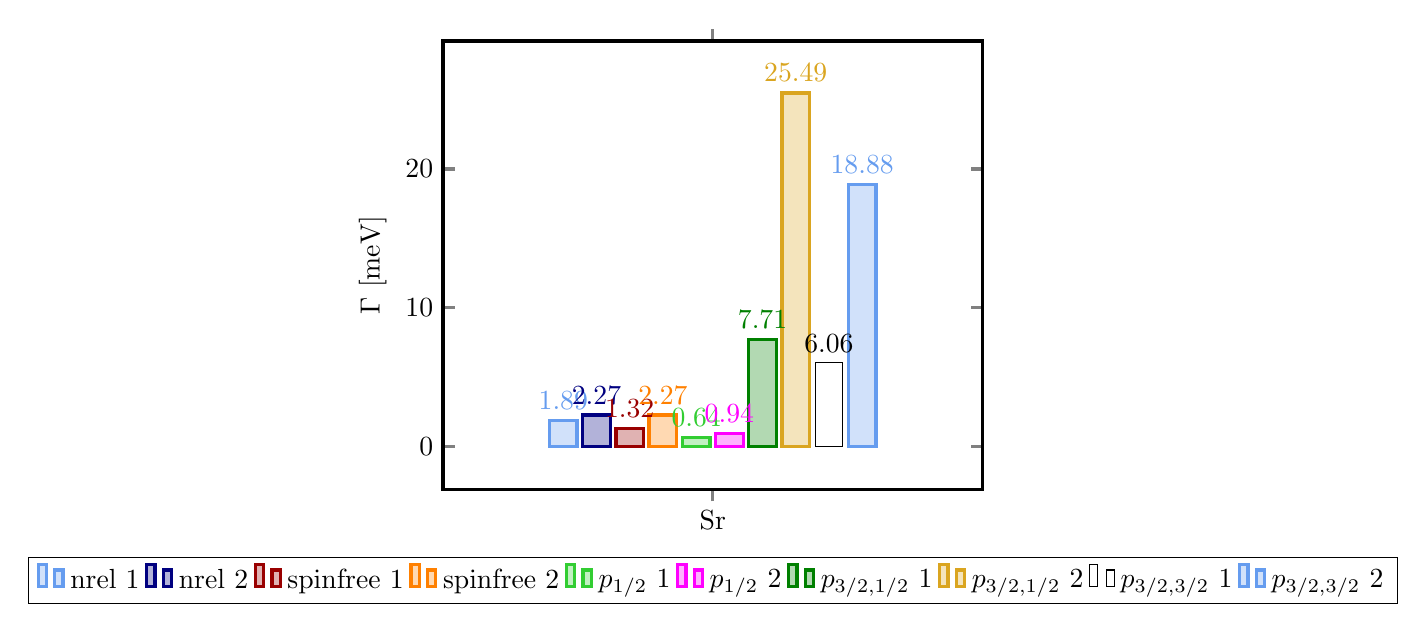
\begin{tikzpicture}
\begin{axis}[
    ybar,
    enlargelimits=0.15,
    legend style={at={(0.5,-0.15)},
      anchor=north,legend columns=-1},
    ylabel={$\Gamma$ [meV]},
    %ylabel={\#participants},
    symbolic x coords={Sr},
    xtick=data,
    nodes near coords,
    nodes near coords align={vertical},
    enlarge x limits=0.25, %space left and right
    axis line style = very thick,
    tick style = very thick
    ]
\addplot coordinates {(Sr,1.888)};
\addplot coordinates {(Sr,2.274)};
\addplot coordinates {(Sr,1.321)};
\addplot coordinates {(Sr,2.269)};
\addplot coordinates {(Sr,0.635)};
\addplot coordinates {(Sr,0.940)};
\addplot coordinates {(Sr,7.712)};
\addplot coordinates {(Sr,25.49)};
\addplot coordinates {(Sr,6.064)};
\addplot coordinates {(Sr,18.88)};
\legend{nrel 1,nrel 2,spinfree 1,spinfree 2,$p_{1/2}$ 1,$p_{1/2}$ 2,$p_{3/2,1/2}$ 1,$p_{3/2,1/2}$ 2,$p_{3/2,3/2}$ 1,$p_{3/2,3/2}$ 2};
\end{axis}
\end{tikzpicture}

\\
%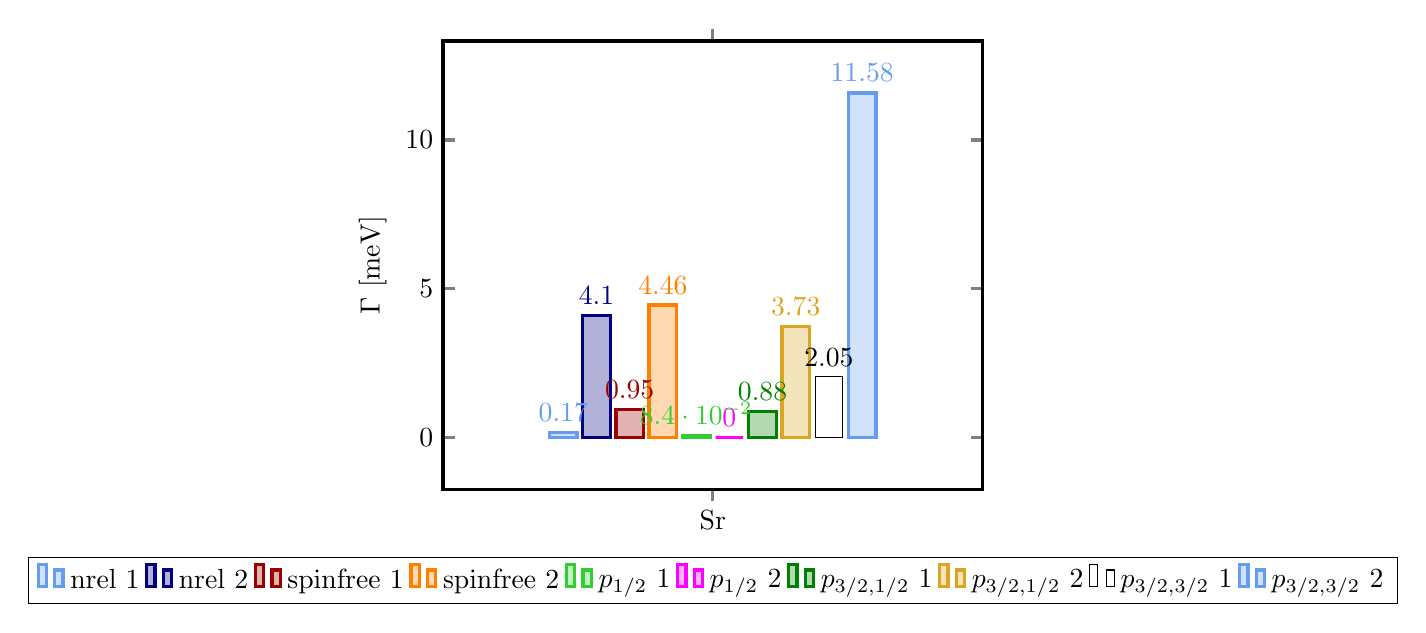
\begin{tikzpicture}
\begin{axis}[
    ybar,
    enlargelimits=0.15,
    legend style={at={(0.5,-0.15)},
      anchor=north,legend columns=-1},
    ylabel={$\Gamma$ [meV]},
    %ylabel={\#participants},
    symbolic x coords={Sr},
    xtick=data,
    nodes near coords,
    nodes near coords align={vertical},
    enlarge x limits=0.25, %space left and right
    axis line style = very thick,
    tick style = very thick
    ]
\addplot coordinates {(Sr,0.170)};
\addplot coordinates {(Sr,4.097)};
\addplot coordinates {(Sr,0.946)};
\addplot coordinates {(Sr,4.460)};
\addplot coordinates {(Sr,0.084)};
\addplot coordinates {(Sr,0.000)};
\addplot coordinates {(Sr,0.878)};
\addplot coordinates {(Sr,3.727)};
\addplot coordinates {(Sr,2.048)};
\addplot coordinates {(Sr,11.58)};
\legend{nrel 1,nrel 2,spinfree 1,spinfree 2,$p_{1/2}$ 1,$p_{1/2}$ 2,$p_{3/2,1/2}$ 1,$p_{3/2,1/2}$ 2,$p_{3/2,3/2}$ 1,$p_{3/2,3/2}$ 2};
\end{axis}
\end{tikzpicture}

\\

%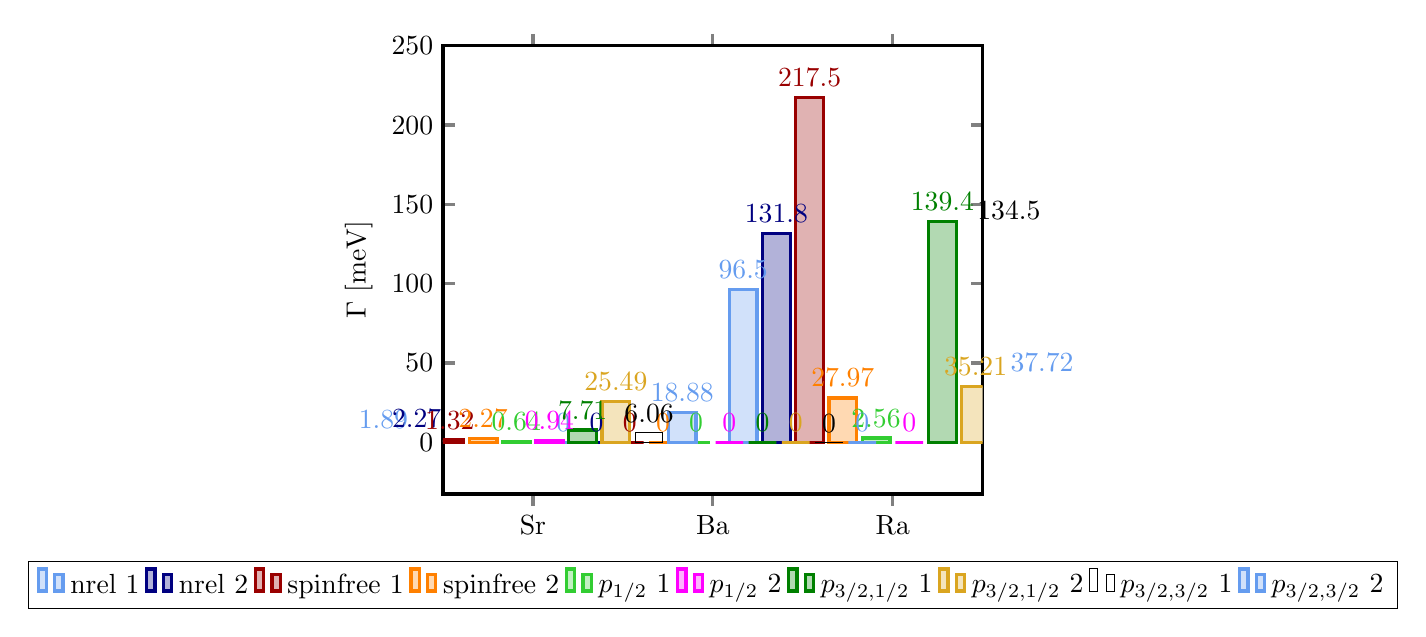
\begin{tikzpicture}
\begin{axis}[
    ybar,
    enlargelimits=0.15,
    legend style={at={(0.5,-0.15)},
      anchor=north,legend columns=-1},
    ylabel={$\Gamma$ [meV]},
    %ylabel={\#participants},
    symbolic x coords={Sr,Ba,Ra},
    xtick=data,
    nodes near coords,
    nodes near coords align={vertical},
    enlarge x limits=0.25, %space left and right
    axis line style = very thick,
    tick style = very thick
    ]
\addplot coordinates {(Sr,1.888) (Ba,0) (Ra,96.50)};
\addplot coordinates {(Sr,2.274) (Ba,0) (Ra,131.8)};
\addplot coordinates {(Sr,1.321) (Ba,0) (Ra,217.5)};
\addplot coordinates {(Sr,2.269) (Ba,0) (Ra,27.97)};
\addplot coordinates {(Sr,0.635) (Ba,0) (Ra,2.564)};
\addplot coordinates {(Sr,0.940) (Ba,0) (Ra,0)};
\addplot coordinates {(Sr,7.712) (Ba,0) (Ra,139.4)};
\addplot coordinates {(Sr,25.49) (Ba,0) (Ra,35.21)};
\addplot coordinates {(Sr,6.064) (Ba,0) (Ra,134.5)};
\addplot coordinates {(Sr,18.88) (Ba,0) (Ra,37.72)};
\legend{nrel 1,nrel 2,spinfree 1,spinfree 2,$p_{1/2}$ 1,$p_{1/2}$ 2,$p_{3/2,1/2}$ 1,$p_{3/2,1/2}$ 2,$p_{3/2,3/2}$ 1,$p_{3/2,3/2}$ 2};
\end{axis}
\end{tikzpicture}

\\
%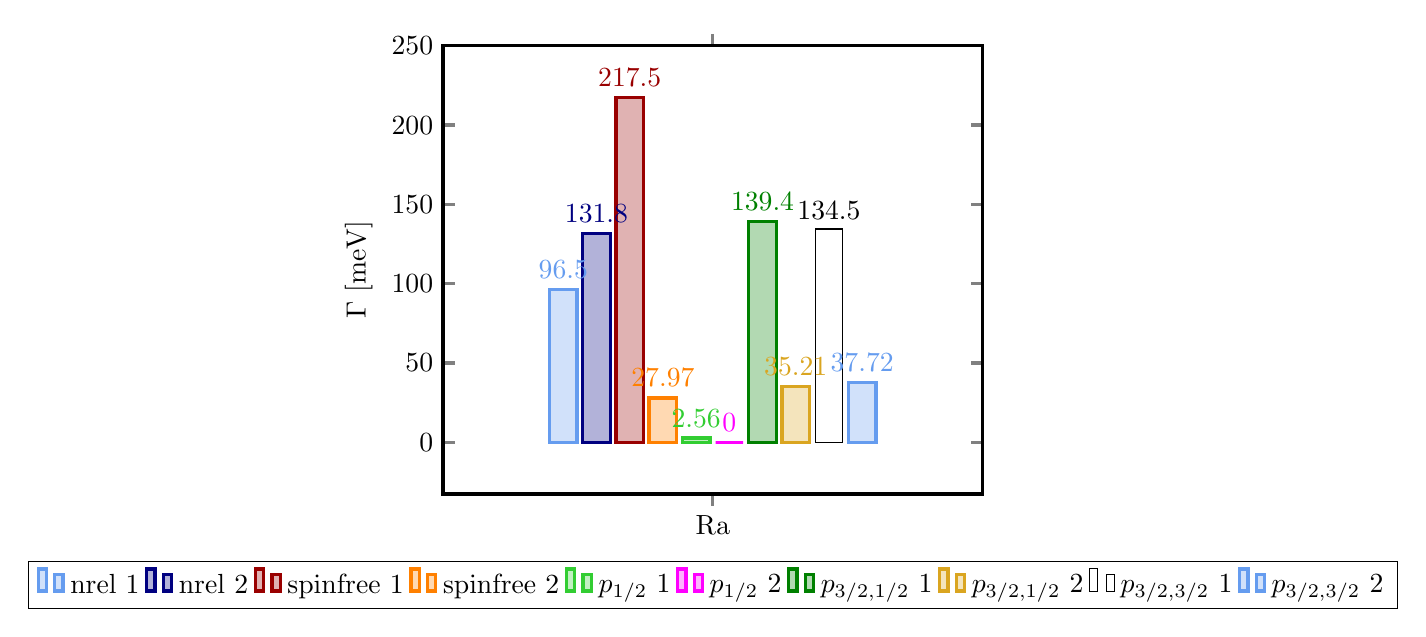
\begin{tikzpicture}
\begin{axis}[
    ybar,
    enlargelimits=0.15,
    legend style={at={(0.5,-0.15)},
      anchor=north,legend columns=-1},
    ylabel={$\Gamma$ [meV]},
    %ylabel={\#participants},
    symbolic x coords={Ra},
    xtick=data,
    nodes near coords,
    nodes near coords align={vertical},
    enlarge x limits=0.25, %space left and right
    axis line style = very thick,
    tick style = very thick
    ]
\addplot coordinates {(Ra,96.50)};
\addplot coordinates {(Ra,131.8)};
\addplot coordinates {(Ra,217.5)};
\addplot coordinates {(Ra,27.97)};
\addplot coordinates {(Ra,2.564)};
\addplot coordinates {(Ra,0)};
\addplot coordinates {(Ra,139.4)};
\addplot coordinates {(Ra,35.21)};
\addplot coordinates {(Ra,134.5)};
\addplot coordinates {(Ra,37.72)};
\legend{nrel 1,nrel 2,spinfree 1,spinfree 2,$p_{1/2}$ 1,$p_{1/2}$ 2,$p_{3/2,1/2}$ 1,$p_{3/2,1/2}$ 2,$p_{3/2,3/2}$ 1,$p_{3/2,3/2}$ 2};
\end{axis}
\end{tikzpicture}

\\
%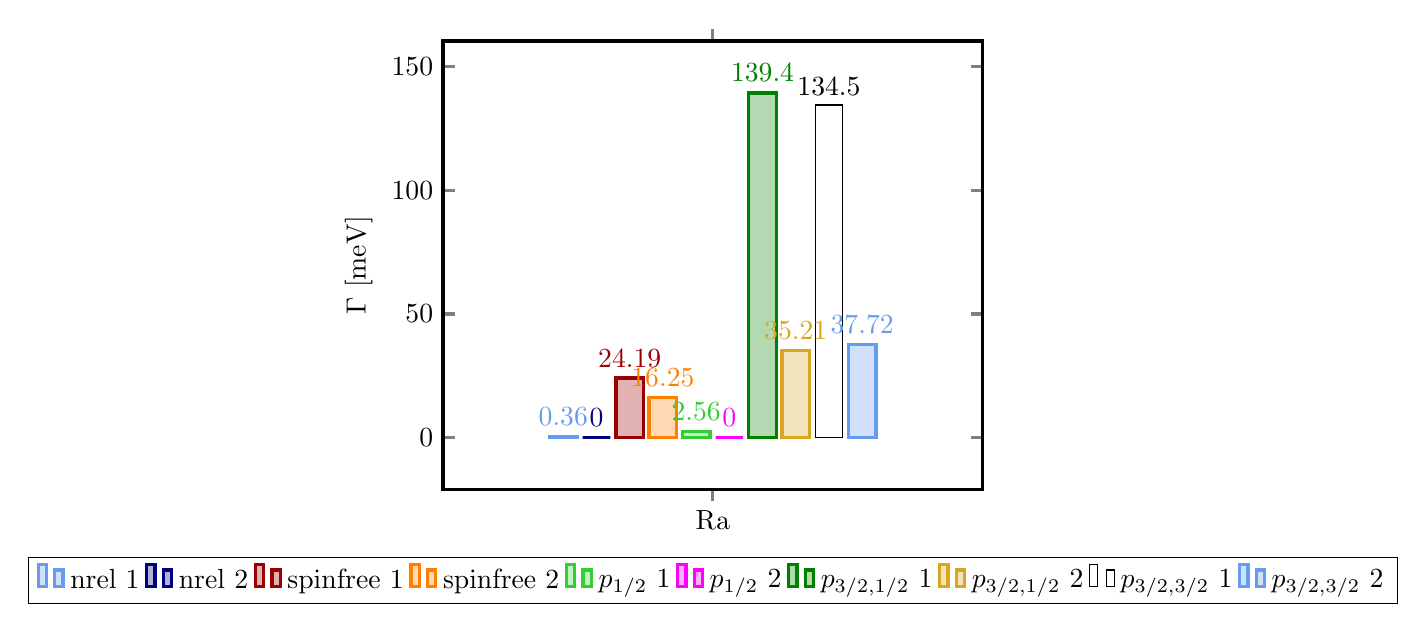
\begin{tikzpicture}
\begin{axis}[
    ybar,
    enlargelimits=0.15,
    legend style={at={(0.5,-0.15)},
      anchor=north,legend columns=-1},
    ylabel={$\Gamma$ [meV]},
    %ylabel={\#participants},
    symbolic x coords={Ra},
    xtick=data,
    nodes near coords,
    nodes near coords align={vertical},
    enlarge x limits=0.25, %space left and right
    axis line style = very thick,
    tick style = very thick
    ]
\addplot coordinates {(Ra,0.358)};
\addplot coordinates {(Ra,0.000)};
\addplot coordinates {(Ra,24.19)};
\addplot coordinates {(Ra,16.25)};
\addplot coordinates {(Ra,2.564)};
\addplot coordinates {(Ra,0)};
\addplot coordinates {(Ra,139.4)};
\addplot coordinates {(Ra,35.21)};
\addplot coordinates {(Ra,134.5)};
\addplot coordinates {(Ra,37.72)};
\legend{nrel 1,nrel 2,spinfree 1,spinfree 2,$p_{1/2}$ 1,$p_{1/2}$ 2,$p_{3/2,1/2}$ 1,$p_{3/2,1/2}$ 2,$p_{3/2,3/2}$ 1,$p_{3/2,3/2}$ 2};
\end{axis}
\end{tikzpicture}


%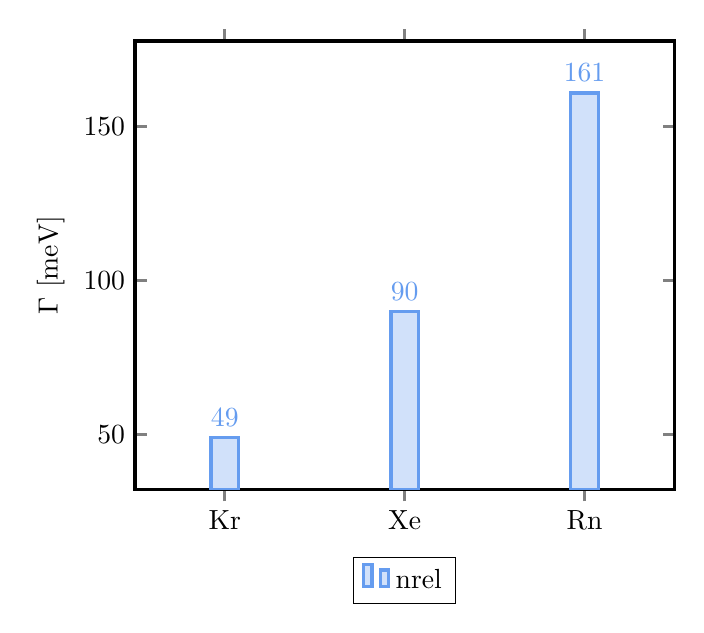
\begin{tikzpicture}
\begin{axis}[
    ybar,
    enlargelimits=0.15,
    legend style={at={(0.5,-0.15)},
      anchor=north,legend columns=-1},
    ylabel={$\Gamma$ [meV]},
    %ylabel={\#participants},
    symbolic x coords={Kr,Xe,Rn},
    xtick=data,
    nodes near coords,
    nodes near coords align={vertical},
    enlarge x limits=0.25, %space left and right
    axis line style = very thick,
    tick style = very thick
    ]
\addplot coordinates {(Kr,49) (Xe,90) (Rn,161)};
%\addplot coordinates {(Kr,62) (Xe,168) (Rn,686)};
%\addplot coordinates {(Kr,56) (Xe,132) (Rn,547)};
%\addplot coordinates {(Kr,63) (Xe,162) (Rn,624)};
\legend{nrel,spinfree,$d_{3/2}$,$d_{5/2}$}
\end{axis}
\end{tikzpicture}



\begin{tikzpicture}[scale=1.0]

\begin{axis}[%scale=1.5,
             domain=0:2.5,
             restrict expr to domain={x}{0:2.5},
             %restrict expr to domain={y}{1.0E-12:7},
             xlabel={r [\AA]},
             %xtick={30,50,...,170},
             %xticklabels={2,4,6,8,10,12,15,20,25},
             %ytick={-1.0,-0.8,...,1.0},
             %yticklabels={1.0,0.8,0.6,0.4,0.2,0.0,0.2,0.4,0.6,0.8,1.0},
             ylabel={$P(r)^2 + Q(r)^2$},
             scale only axis,
             width=12cm,
             height=8cm,
             %ybar stacked
             cycle list name = diplom,
             legend cell align=right,
             axis line style = very thick,
             tick style = very thick
             ]


\addplot+[
         mark=none,
         %color=diplom1,
         very thick
         ]
         table[
         x expr= 0.529 * (\thisrowno{1}),
         y expr={(\thisrowno{6})^2 + (\thisrowno{7})^2}
         ]
         {../data/sr_4p.dat};
         \addlegendentry{Sr rel. 4$p_{1/2}$};

\addplot+[
         mark=none,
         %color=diplom1,
         very thick
         ]
         table[
         x expr= 0.529 * (\thisrowno{1}),
         y expr={(\thisrowno{8})^2 + (\thisrowno{9})^2}
         ]
         {../data/sr_4p.dat};
         \addlegendentry{Sr rel. 4$p_{3/2}$};

\addplot+[
         mark=none,
         %color=diplom1,
         very thick
         ]
         table[
         x expr= 0.529 * (\thisrowno{1}),
         y expr={(\thisrowno{2})^2 + (\thisrowno{3})^2}
         ]
         {../data/sr_5s.dat};
         \addlegendentry{Sr rel. 5$s$};

%\addplot+[
%         mark=none,
%         %color=diplom2,
%         very thick
%         ]
%         table[
%         x expr= 0.529 * (\thisrowno{1}),
%         y expr={(\thisrowno{4})^2 + (\thisrowno{5})^2}
%         ]
%         {../data/P_xe_nrel_outer.dat};
%         \addlegendentry{Xe nrel. 4d};
%
%
%%s
%\addplot+[
%         mark=none,
%         %color=diplom1,
%         very thick
%         ]
%         table[
%         x expr= 0.529 * (\thisrowno{1}),
%         y expr={(\thisrowno{6})^2 + (\thisrowno{7})^2}
%         ]
%         {../data/P_xe_rel_outer.dat};
%         \addlegendentry{Xe rel. 5s};
%
%\addplot+[
%         mark=none,
%         %color=diplom2,
%         very thick
%         ]
%         table[
%         x expr= 0.529 * (\thisrowno{1}),
%         y expr={(\thisrowno{6})^2 + (\thisrowno{7})^2}
%         ]
%         {../data/P_xe_nrel_outer.dat};
%         \addlegendentry{Xe nrel. 5s};
%
%%p
%\addplot+[
%         mark=none,
%         %color=diplom1,
%         very thick
%         ]
%         table[
%         x expr= 0.529 * (\thisrowno{1}),
%         y expr={(\thisrowno{8})^2 + (\thisrowno{9})^2}
%         ]
%         {../data/P_xe_rel_outer.dat};
%         \addlegendentry{Xe rel. 5p};
%
%\addplot+[
%         mark=none,
%         %color=diplom2,
%         very thick
%         ]
%         table[
%         x expr= 0.529 * (\thisrowno{1}),
%         y expr={(\thisrowno{8})^2 + (\thisrowno{9})^2}
%         ]
%         {../data/P_xe_nrel_outer.dat};
%         \addlegendentry{Xe nrel. 5p};


\end{axis}
\end{tikzpicture}

\begin{tikzpicture}[scale=1.0]

\begin{axis}[%scale=1.5,
             domain=0:2.5,
             restrict expr to domain={x}{0:2.5},
             %restrict expr to domain={y}{1.0E-12:7},
             xlabel={r [\AA]},
             %xtick={30,50,...,170},
             %xticklabels={2,4,6,8,10,12,15,20,25},
             %ytick={-1.0,-0.8,...,1.0},
             %yticklabels={1.0,0.8,0.6,0.4,0.2,0.0,0.2,0.4,0.6,0.8,1.0},
             ylabel={$P(r)^2 + Q(r)^2$},
             scale only axis,
             width=12cm,
             height=8cm,
             %ybar stacked
             cycle list name = diplom,
             legend cell align=right,
             axis line style = very thick,
             tick style = very thick
             ]


\addplot+[
         mark=none,
         %color=diplom1,
         very thick
         ]
         table[
         x expr= 0.529 * (\thisrowno{1}),
         y expr={(\thisrowno{4})^2 + (\thisrowno{5})^2}
         ]
         {../data/ba_5p.dat};
         \addlegendentry{Ba rel. 5$p_{1/2}$};

\addplot+[
         mark=none,
         %color=diplom1,
         very thick
         ]
         table[
         x expr= 0.529 * (\thisrowno{1}),
         y expr={(\thisrowno{2})^2 + (\thisrowno{3})^2}
         ]
         {../data/ba_6s.dat};
         \addlegendentry{Ba rel. 5$p_{3/2}$};

\addplot+[
         mark=none,
         %color=diplom1,
         very thick
         ]
         table[
         x expr= 0.529 * (\thisrowno{1}),
         y expr={(\thisrowno{4})^2 + (\thisrowno{5})^2}
         ]
         {../data/ba_6s.dat};
         \addlegendentry{Ba rel. 6$s$};

%\addplot+[
%         mark=none,
%         %color=diplom2,
%         very thick
%         ]
%         table[
%         x expr= 0.529 * (\thisrowno{1}),
%         y expr={(\thisrowno{4})^2 + (\thisrowno{5})^2}
%         ]
%         {../data/P_xe_nrel_outer.dat};
%         \addlegendentry{Xe nrel. 4d};
%
%
%%s
%\addplot+[
%         mark=none,
%         %color=diplom1,
%         very thick
%         ]
%         table[
%         x expr= 0.529 * (\thisrowno{1}),
%         y expr={(\thisrowno{6})^2 + (\thisrowno{7})^2}
%         ]
%         {../data/P_xe_rel_outer.dat};
%         \addlegendentry{Xe rel. 5s};
%
%\addplot+[
%         mark=none,
%         %color=diplom2,
%         very thick
%         ]
%         table[
%         x expr= 0.529 * (\thisrowno{1}),
%         y expr={(\thisrowno{6})^2 + (\thisrowno{7})^2}
%         ]
%         {../data/P_xe_nrel_outer.dat};
%         \addlegendentry{Xe nrel. 5s};
%
%%p
%\addplot+[
%         mark=none,
%         %color=diplom1,
%         very thick
%         ]
%         table[
%         x expr= 0.529 * (\thisrowno{1}),
%         y expr={(\thisrowno{8})^2 + (\thisrowno{9})^2}
%         ]
%         {../data/P_xe_rel_outer.dat};
%         \addlegendentry{Xe rel. 5p};
%
%\addplot+[
%         mark=none,
%         %color=diplom2,
%         very thick
%         ]
%         table[
%         x expr= 0.529 * (\thisrowno{1}),
%         y expr={(\thisrowno{8})^2 + (\thisrowno{9})^2}
%         ]
%         {../data/P_xe_nrel_outer.dat};
%         \addlegendentry{Xe nrel. 5p};


\end{axis}
\end{tikzpicture}

\begin{tikzpicture}[scale=1.0]

\begin{axis}[%scale=1.5,
             domain=0:2.5,
             restrict expr to domain={x}{0:2.5},
             %restrict expr to domain={y}{1.0E-12:7},
             xlabel={r [\AA]},
             %xtick={30,50,...,170},
             %xticklabels={2,4,6,8,10,12,15,20,25},
             %ytick={-1.0,-0.8,...,1.0},
             %yticklabels={1.0,0.8,0.6,0.4,0.2,0.0,0.2,0.4,0.6,0.8,1.0},
             ylabel={$P(r)^2 + Q(r)^2$},
             scale only axis,
             width=12cm,
             height=8cm,
             %ybar stacked
             cycle list name = diplom,
             %cycle list name = exotic,
             legend cell align=right,
             axis line style = very thick,
             tick style = very thick
             ]


\addplot+[
         mark=none,
         %color=diplom1,
         very thick
         ]
         table[
         x expr= 0.529 * (\thisrowno{1}),
         y expr={(\thisrowno{4})^2 + (\thisrowno{5})^2}
         ]
         {../data/ra_6p.dat};
         \addlegendentry{Ra rel. 6$p_{1/2}$};

\addplot+[
         mark=none,
         %color=diplom1,
         very thick
         ]
         table[
         x expr= 0.529 * (\thisrowno{1}),
         y expr={(\thisrowno{6})^2 + (\thisrowno{7})^2}
         ]
         {../data/ra_6p.dat};
         \addlegendentry{Ra rel. 6$p_{3/2}$};

\addplot+[
         mark=none,
         %color=diplom1,
         very thick
         ]
         table[
         x expr= 0.529 * (\thisrowno{1}),
         y expr={(\thisrowno{2})^2 + (\thisrowno{3})^2}
         ]
         {../data/ra_7s.dat};
         \addlegendentry{Ra rel. 7$s$};

%\addplot+[
%         mark=none,
%         %color=diplom2,
%         very thick
%         ]
%         table[
%         x expr= 0.529 * (\thisrowno{1}),
%         y expr={(\thisrowno{4})^2 + (\thisrowno{5})^2}
%         ]
%         {../data/P_xe_nrel_outer.dat};
%         \addlegendentry{Xe nrel. 4d};
%
%
%%s
%\addplot+[
%         mark=none,
%         %color=diplom1,
%         very thick
%         ]
%         table[
%         x expr= 0.529 * (\thisrowno{1}),
%         y expr={(\thisrowno{6})^2 + (\thisrowno{7})^2}
%         ]
%         {../data/P_xe_rel_outer.dat};
%         \addlegendentry{Xe rel. 5s};
%
%\addplot+[
%         mark=none,
%         %color=diplom2,
%         very thick
%         ]
%         table[
%         x expr= 0.529 * (\thisrowno{1}),
%         y expr={(\thisrowno{6})^2 + (\thisrowno{7})^2}
%         ]
%         {../data/P_xe_nrel_outer.dat};
%         \addlegendentry{Xe nrel. 5s};
%
%%p
%\addplot+[
%         mark=none,
%         %color=diplom1,
%         very thick
%         ]
%         table[
%         x expr= 0.529 * (\thisrowno{1}),
%         y expr={(\thisrowno{8})^2 + (\thisrowno{9})^2}
%         ]
%         {../data/P_xe_rel_outer.dat};
%         \addlegendentry{Xe rel. 5p};
%
%\addplot+[
%         mark=none,
%         %color=diplom2,
%         very thick
%         ]
%         table[
%         x expr= 0.529 * (\thisrowno{1}),
%         y expr={(\thisrowno{8})^2 + (\thisrowno{9})^2}
%         ]
%         {../data/P_xe_nrel_outer.dat};
%         \addlegendentry{Xe nrel. 5p};


\end{axis}
\end{tikzpicture}


\end{document}
